%%%%%%%%%%%%%%%%%%%%%%%%%%%%%%%%%%%%%%%%%%%%%%%%%%%%%%%%%%%%%%%%%%%%%%%%

%%% LaTeX Template for AAMAS-2024 (based on sample-sigconf.tex)
%%% Prepared by the AAMAS-2024 Program Chairs based on the version from AAMAS-2023. 

%%%%%%%%%%%%%%%%%%%%%%%%%%%%%%%%%%%%%%%%%%%%%%%%%%%%%%%%%%%%%%%%%%%%%%%%

%%% Start your document with the \documentclass command.


%%% == IMPORTANT ==
%%% Use the first variant below for the final paper (including auithor information).
%%% Use the second variant below to anonymize your submission (no authoir information shown).
%%% For further information on anonymity and double-blind reviewing, 
%%% please consult the call for paper information
%%% https://www.aamas2024-conference.auckland.ac.nz/calls/submission-instruction/

\documentclass[sigconf]{aamas} 
%\documentclass[sigconf,anonymous]{aamas} 


%%% Load required packages here (note that many are included already).

\usepackage{balance} % for balancing columns on the final page

%%%%%%%%%%%%%%%%%%%%%%%%%%%%%%%%%%%%%%%%%%%%%%%%%%%%%%%%%%%%%%%%%%%%%%%%

%%% AAMAS-2024 copyright block (do not change!)

\setcopyright{ifaamas}
\acmConference[AAMAS '24]{Proc.\@ of the 23rd International Conference
on Autonomous Agents and Multiagent Systems (AAMAS 2024)}{May 6 -- 10, 2024}
{Auckland, New Zealand}{N.~Alechina, V.~Dignum, M.~Dastani, J.S.~Sichman (eds.)}
\copyrightyear{2024}
\acmYear{2024}
\acmDOI{}
\acmPrice{}
\acmISBN{}

%%%%%%%%%%%%%%%%%%%%%%%%%%%%%%%%%%%%%%%%%%%%%%%%%%%%%%%%%%%%%%%%%%%%%%%%

%%% == IMPORTANT ==
%%% Use this command to specify your EasyChair submission number.
%%% In anonymous mode, it will be printed on the first page.

\acmSubmissionID{<<EasyChair submission id>>}

%%% Use this command to specify the title of your paper.

\title[AAMAS-2024 CybMASDE]{CybMASDE: A Development Environment For Cyberdefense Multi-Agent Systems}

%%% Provide names, affiliations, and email addresses for all authors.

\author{Julien Soulé}
\affiliation{
  \institution{Univ. Grenoble Alpes}
  \city{Valence}
  \country{France}}
\email{julien.soule@lcis.grenoble-inp.fr}

\author{Jean-Paul Jamont}
\affiliation{
  \institution{Univ. Grenoble Alpes}
  \city{Valence}
  \country{France}}
\email{jean-paul.jamont@lcis.grenoble-inp.fr}

\author{Michel Occello}
\affiliation{
  \institution{Univ. Grenoble Alpes}
  \city{Valence}
  \country{France}}
\email{michel.occello@lcis.grenoble-inp.fr}

\author{Louis-Marie Traonouez}
\affiliation{
  \institution{Thales Land and Air Systems, BU IAS}
  \city{Rennes}
  \country{France}}
\email{louis-marie.traonouez@thalesgroup.com}

\author{Paul Théron}
\affiliation{
  \institution{AICA IWG}
  \city{La Guillermie}
  \country{France}}
\email{paul.theron@orange.fr}

%%% Use this environment to specify a short abstract for your paper.

% ----------------------------------
%   Notes
% ----------------------------------

% Novel applications and interactive systems are particularly welcome.

% Demonstrations of interest include:
%   - Systems implementing agents in real-world applications in areas such as transportation, robotics, grid, e-commerce, health care, military, etc.
%   - Systems using agents in virtual settings, which include simulation systems, VR, and games.
%   - Systems supporting the development of agents, which include development environments and tools to assist developers in the specification, design, implementation, and testing of agent systems.


% Each Demo submission must consist of a short paper, a video, and, for student projects, a supervisor endorsement note. The submission requirements are the following.

% 1. Paper. The paper should include a maximum of four pages and be structured as follows:
% - Pages 1-2 should describe the system to be demonstrated. More precisely, the authors are encouraged to discuss the application domain, the problem scenario, the technology used, the agent/multi-agent techniques involved, the system’s innovations, the system’s live and interactive aspects, etc.
% - Page 3 should include bibliographic references.
% - Page 4 should provide the organisers with a list of requirements for the demo setting at the conference.

% 2. Video. The paper should contain a URL linking to a demonstration video of no more than 5 minutes in duration (QuickTime or YouTube format). The video should include the following elements:
% - Introduction: Introduce the concept/system.
% - Aim: What is the target group for the system?
% - Main features: Present the system’s main features and discuss the benefits as well as innovations.
% - Development: Architecture overview, agent-based techniques, and technologies used for development.
% - Demo. Execution of the system that highlights its features and benefits.

% The evaluation criteria are:
% - Relevance to the AAMAS conference
% - Significance and originality
% - Live demo presentation and technical quality
% - Video content and presentation
% - Maturity and readiness for demonstration
% - Potential for public interaction
% - Potential impact in the intended application domain

% ----------------------------------


\begin{abstract}
We present N eSSi2 , the Network Security Simulator, a simulation environment that is based on the service-centric agent platform JIAC. It focuses on network security-related scenarios such as attack analysis and evaluation of countermeasures. We introduce the main N eSSi2 concepts and discuss the motivation for realizing them with agent technology. Then, we present the individual components and examples where N eSSi2 has been successfully applied.
\end{abstract}

%%% The code below was generated by the tool at http://dl.acm.org/ccs.cfm.
%%% Please replace this example with code appropriate for your own paper.


%%% Use this command to specify a few keywords describing your work.
%%% Keywords should be separated by commas.

\keywords{Cyberdefense, Multiagent systems, Design tool, Network application-level, Simulation, Emulation, Demo}

%%%%%%%%%%%%%%%%%%%%%%%%%%%%%%%%%%%%%%%%%%%%%%%%%%%%%%%%%%%%%%%%%%%%%%%%

%%% Include any author-defined commands here.
         
\newcommand{\BibTeX}{\rm B\kern-.05em{\sc i\kern-.025em b}\kern-.08em\TeX}

%%%%%%%%%%%%%%%%%%%%%%%%%%%%%%%%%%%%%%%%%%%%%%%%%%%%%%%%%%%%%%%%%%%%%%%%

\begin{document}

%%% The following commands remove the headers in your paper. For final 
%%% papers, these will be inserted during the pagination process.

\pagestyle{fancy}
\fancyhead{}

%%% The next command prints the information defined in the preamble.

\maketitle 

%%%%%%%%%%%%%%%%%%%%%%%%%%%%%%%%%%%%%%%%%%%%%%%%%%%%%%%%%%%%%%%%%%%%%%%%

\section{Introduction}

The design and development of security solutions such as Intrusion Detection Systems (IDS) is a challenging and complex task. In this process, the evolving system needs to be evaluated continuously. There are several ways to study a system or technology. The most accurate is the analysis of the deployed production system. However, in the case of IDS evaluation, real experiments incorporating attack scenarios cannot be done in an operational environment because the induced risk of failures such as service loss is too high.

For this very reason, evaluation is often carried out in small testbeds. Virtual machines are a solution for modeling mid-scale networks, but the representation of very large networks with thousands or millions of devices and links is out of scope. There exist scientific initiatives such as PlanetLab1 providing computational resources to a larger extent.
This is an important opportunity for researchers to evaluate network or security functionality, but although they provide detailed results, experiments are time consuming and remain complex to setup and maintain.

% \begin{table}[t]
% 	\caption{Locations of the first five editions of AAMAS}
% 	\label{tab:locations}
% 	\begin{tabular}{rll}\toprule
% 		\textit{Year} & \textit{City} & \textit{Country} \\ \midrule
% 		2002 & Bologna & Italy \\
% 		2003 & Melbourne & Australia \\
% 		2004 & New York City & USA \\
% 		2005 & Utrecht & The Netherlands \\
% 		2006 & Hakodate & Japan \\ \bottomrule
% 	\end{tabular}
% \end{table}

Another approach is to represent the system with the aid of mathematical models and find analytical answers, i.e. logical and quantitative relationships between the entities.
Typically, such models also become very complex, in particular for a concurrent system such as IDS. Therefore, simulations are useful for the evaluation of distributed systems and protocols. Depending on the evaluation metrics, the simulations allow the abstraction from irrelevant properties.
In addition, hazard scenarios, called “what-if scenarios”, can be constructed which may not be possible in real-world test environments.


%%%%%%%%%%%%%%%%%%%%%%%%%%%%%%%%%%%%%%%%%%%%%%%%%%%%%%%%%%%%%%%%%%%%%%%%

\section{Solution approach}

We introduce N eSSi2 , an agent-based simulation environment [3], providing telecommunication network simulation capabilities with an extensive support to evaluate security solutions such as IDS. In contrast to other network simulators, like e.g. NS-3 [2], N eSSi2 also provides a comprehensive detection API for the integration and evaluation of IDS. In particular, special common attack scenarios can be simulated. Worm-spread scenarios and botnet-based DDoS attacks are only two of the supported example attacks. In
addition, customized profiles defining the node behavior can be applied within the simulation.

N eSSi2 is built upon the JIAC [1] framework, a service-centric agent-framework. The most recent version, JIAC V2 , is used in N eSSi2 . The network entities, i.e. routers, clients, servers, or IDS (nodes in the following) are simulated with the aid of JIAC agents. Dependent on configuration parameters and hardware characteristics, each agent simulates one or more nodes. N eSSi2 is benefiting from agent technology in general and JIAC in special through the service-centric, modular and flexible approach to realizing distributed execution environments. In addition, a common semantic data model enables interoperability of agents executing even different simulation models at the same time.

This semantic model also incorporates the main modeling concepts for the creation and administration of simulations.
The first concept and step to setup a simulation is the creation of the network topology. This topology can then be re-used for different scenarios. The scenario is comprised of elementary building blocks for each device in the network, the node profiles. They allow the customization of node behavior to automatically generate traffic, simulate failures or apply network-based defense measures. Every profile consists of applications, representing mechanisms to be executed on an individual node, e.g. an attack, a detection mechanism or an application protocol such as HTTP. The sum of all profiles for a given network is called the scenario. In order to execute it, the length of simulation execution, the number of simulation runs and a recording configuration are configured within a session. As simulations often contain stochastical components such as distribution functions, e.g. the number/timing of HTTP-requests, multiple runs allow for the statistical analysis of mean values and standard deviations.

%%%%%%%%%%%%%%%%%%%%%%%%%%%%%%%%%%%%%%%%%%%%%%%%%%%%%%%%%%%%%%%%%%%%%%%%

\section{Architecture}

N eSSi2 has been structured into three distinct components, the graphical frontend, the agent-based simulation backend and the result database. Each of these modules may be run on separate machines. The modular design facilitates the exchange of network topologies, scenario definitions and simulation results.

The graphical frontend of N eSSi2 (c.f. Figure1) allows to create and edit the necessary components of a network simulation as described in Section 2. On the other hand, finished (or even currently executing, long-running) simulations can be retrieved from the database server and the corresponding simulation results are visualized in the GUI. Accordingly, there exist two different perspectives in the GUI, the Network Editor perspective for the creation of simulations as well as the Network Simulation perspective to investigate simulation results.

In the backend, different agent roles carry out the task of the parallel simulation execution. On each backend, i.e. separate machine, there exists the Simulation Control Agent (SCA) administrating access to the resources of the system as well as the interaction with the GUI. In this way, the SCA interacts with the individual Network Simulation Coordination Agents (NCAs). For every executed simulation run, an NCA is invoked which starts a number of Device Management Agents (DMAs). The number of DMAs depends either on particular user configurations, e.g. “one agent for every node”, “x agents in total”, or follows the computational power of the backend system, i.e. “one agent per CPU core”.

Finally, the result database stores simulation results according to the configuration specified during the creation process of the simulation in the GUI. For every simulation run, the agents record selected events and traffic data to a specified log4j3 appender which handles the output according to the recorder configuration. By default, the results – such as attack-related events – as well as the model are recorded to a database which allows for replaying the simulation. In addition, the recorded data can be used for
evaluation purposes.

\begin{figure}[h]
  \centering
  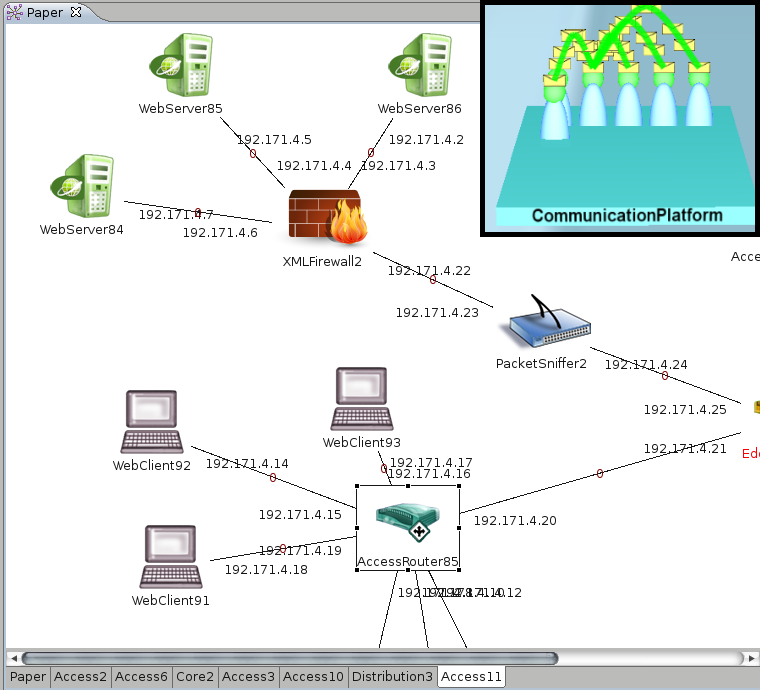
\includegraphics[width=\linewidth]{screenshot.png}
  \caption{Main view in NeSSi2: The GUI enables the creation and administration of arbitrary networks and node configurations. After the setup process is finished, an agent-based simulation back-end (“CommunicationPlatform”) executes the simulation and the results are stored in a database.}
  \label{fig:screenshot}
  \Description{Screenshot of the main view in NeSSi2: The GUI enables the creation and administration of arbitrary networks and node configurations. After the setup process is finished, an agent-based simulation back-end (“CommunicationPlatform”) executes the simulation and the results are stored in a database.}
\end{figure}

%%%%%%%%%%%%%%%%%%%%%%%%%%%%%%%%%%%%%%%%%%%%%%%%%%%%%%%%%%%%%%%%%%%%%%%%

\section{Successful utilization}

N eSSi2 has demonstrated its value in recent research and was employed as a simulation environment for various security-related approaches. In this regard, N eSSi2 was used to investigate optimal placement strategies for IDS, analyze worm propagation strategies and evaluate the benefit of collaborative IDS. N eSSi2 has also been used in lectures to generate attack data and evaluate detection algorithms implemented by students. In a recent industry research project, N eSSi2 has been incorporated in an agent-based Decision Support System to forecast upcoming link congestions in the access network of a big German DSL-provider.
N eSSi2 is Open Source since January of 2009 and has been
downloaded more than 6000 times.

%%%%%%%%%%%%%%%%%%%%%%%%%%%%%%%%%%%%%%%%%%%%%%%%%%%%%%%%%%%%%%%%%%%%%%%%

\section{Conclusion}

We have presented N eSSi2 , a network simulation environment with a focus on security-related scenarios. The simulation backend is based on agent technology benefiting from the service-centric, modular and flexible design of the JIAC framework to load balance the complexity of the simulation runs. N eSSi2 incorporates a semantic data model to reflect simulations of arbitrary networks and individual node configurations and has been used in various (industry) research projects as well as lectures. Related publications, documentation and source code can be looked up on the web site, c.f. http://www.nessi2.de.\nocite{*}

%%%%%%%%%%%%%%%%%%%%%%%%%%%%%%%%%%%%%%%%%%%%%%%%%%%%%%%%%%%%%%%%%%%%%%%% 

% TODO: ?
% \begin{acks}
% \end{acks}

%%%%%%%%%%%%%%%%%%%%%%%%%%%%%%%%%%%%%%%%%%%%%%%%%%%%%%%%%%%%%%%%%%%%%%%%

\newpage

\bibliographystyle{ACM-Reference-Format} 
\bibliography{sample}

%%%%%%%%%%%%%%%%%%%%%%%%%%%%%%%%%%%%%%%%%%%%%%%%%%%%%%%%%%%%%%%%%%%%%%%%

\newpage
\phantom{ }
\newpage

\section*{Requirements for the demo setting}




%%%%%%%%%%%%%%%%%%%%%%%%%%%%%%%%%%%%%%%%%%%%%%%%%%%%%%%%%%%%%%%%%%%%%%%%

\end{document}

%%%%%%%%%%%%%%%%%%%%%%%%%%%%%%%%%%%%%%%%%%%%%%%%%%%%%%%%%%%%%%%%%%%%%%%%

